\begin{frame}{\(\DConf_2(K_5)\) is a surface}

\begin{columns}[T,onlytextwidth]
	\begin{column}{0.5\textwidth}
		\centering
        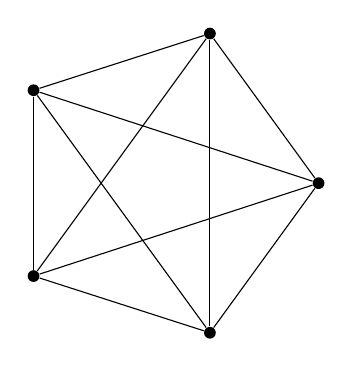
\begin{tikzpicture}[scale=2]
            \node[circle, fill, inner sep=1.5pt] (v1) at (1, 0) {};
            \node[circle, fill, inner sep=1.5pt] (v2) at (.31, .95) {};
            \node[circle, fill, inner sep=1.5pt] (v3) at (-.81, .59) {};
            \node[circle, fill, inner sep=1.5pt] (v4) at (-.81, -.59) {};
            \node[circle, fill, inner sep=1.5pt] (v5) at (0.31,  -0.95) {};
            
            \draw (v1) -- (v2);
            \draw (v1) -- (v3);
            \draw (v1) -- (v4);
            \draw (v1) -- (v5);
            \draw (v2) -- (v3);
            \draw (v2) -- (v4);
            \draw (v2) -- (v5);
            \draw (v3) -- (v4);
            \draw (v3) -- (v5);
            \draw (v4) -- (v5);
        \end{tikzpicture}
        
        \vspace{1em}
		\scriptsize \(K_5\)
	\end{column}

	\begin{column}{0.5\textwidth}
		\centering
        \vspace{9.5em}
        \url{https://skfb.ly/AYo8}

		\scriptsize

        \vspace{1em}
        Michelle Chu's model of \(\DConf_2(K_5)\)
    \end{column}
\end{columns}
\end{frame}